\documentclass[12pt]{article}
\usepackage[utf8]{inputenc}
\usepackage{sbc-template}
\usepackage{multirow}
\usepackage{graphicx,url}
\usepackage{placeins}
\usepackage{float}

%\usepackage[brazil]{babel}   


     
\sloppy

\title{Uma Solução para Comunicação Criptografada entre Dispositivos \textbf{\textit{IoT}}}

\author{Erik Henrique de Oliveira Zambeli - RA: 1749927}


\address{Universidade Tecnológica Federal do Paraná (UTFPR)\\
  Campus Cornélio Procópio -- PR -- Brazil
}

\begin{document} 

\maketitle

\begin{abstract}
 Observing the technological evolution and the constant use of devices connected to computing and the Internet, the security challenges in the so-called Internet of Things are studied. This work presents briefly the problems of security and internet communication of things. Many people do not realize how much personal data pertaining to their lives and their daily lives pass through the internet, much of this data may be vulnerable to various attacks, another point to note is that before these attacks devices that were previously designed for a specific function may exhibit distinct behavior by exposing the users' privacy. The article will introduce key cryptographic algorithms for data protection and provide a solution for encrypted communication for devices connected to the Internet.



\textbf{Keywords:} Security, Protocols, Internet of Things, Encryption, Communication, Algorithms.
\end{abstract}
     
\begin{resumo} 
  Observando a evolução tecnológica e o uso constante de dispositivos ligados a computação e a Internet, são estudados os desafios da segurança na chamada \textbf{\textit{IoT}}. Este trabalho apresenta de forma breve os problemas de segurança e comunicação pela \textbf{\textit{IoT}}. Muitas pessoas não percebem o quanto de dados pessoais relativos a sua vida e o seu dia-a-dia transita pela internet, muito desses dados podem estar vulneráveis a ataques diversos, outro ponto a se destacar é que diante desses ataques aparelhos que antes eram projetados para uma função especifica podem apresentar comportamento distinto expondo a privacidade dos usuários. O artigo fara a apresentação dos principais algoritmos de criptografia para proteção de dados e apresentara uma solução para a comunicação criptografada para dispositivos conectados a internet.  


\textbf{Palavras-chave:} Segurança, Protocolos, Internet das Coisas, Criptografia, Comunicação, Algoritmos.  

\end{resumo}


\section{Introdução}

A Internet das Coisas (em inglês: Internet of Things , abreviadamente, \textbf{\textit{IoT}}) é um conceito que se refere à conexão digital de objetos cotidianos com a internet. Em outras palavras, a \textbf{\textit{IoT}} nada mais é que uma rede de objetos físicos (veículos, prédios, sensores, TVs, geladeiras, carros, etc...), é uma extensão da internet atual que possibilita que objetos do dia-a-dia que possuam capacidade computacional e de comunicação se conectem com a internet. A conexão com a rede mundial de computadores possibilita, controle remoto dos objetos e, que os próprios objetos sejam acessados como provedores de serviços. Entretanto toda essa tecnologia remete grandes preocupações da forma como as informações podem estar vulneráveis a interceptações. 


A \textbf{\textit{IoT}} promete uma comodidade incomparável. Porém, para que a \textbf{\textit{IoT}} atinja seu potencial, é essencial conquistar e manter a confiança do consumidor sobre questões como privacidade e segurança. Os dados transmitidos pela \textbf{\textit{IoT}} formão uma compilação de cada um dos usuários e aplicações e hardwares trazem sérios riscos se não forem desenvolvidos levando-se em consideração questões de segurança da informação colhida, tratada e transmitida.


Os dados gerados pelos diversos dispositivos que compõem a \textbf{\textit{IoT}} passam por diversas redes e muitas vezes passam por aplicativos móveis e são armazenados na nuvem. Há então uma preocupação relacionada à privacidade, já que os dados passam por diferentes ambientes que fogem do controle do usuário. Garantir que o transporte de dados terá confidencialidade, integridade, autenticação dos envolvidos e garantia de irretratabilidade são os principais objetivos da criptografia, objetivos estes fundamentais para um transporte de dados seguro.


Portanto o presente artigo pretende abordar o conceito da segurança, o básico relacionado à encriptação com foco em sigilo de dados. Além disso, apresenta uma aplicação para comunicação criptografada entre diferentes dispositivos e aplicações.

A primeira seção faz uma contextualização de \textbf{\textit{IoT}} e apresenta a importância da comunicação segura entre dispositivos conectados. A segunda seção aborda os conceitos de criptografia e apresenta de forma conceitual os algoritmos de criptografia simétricos e assimétricos mais comuns na internet. A terceira seção algumas soluções de mercado presentes hoje em dia que buscam solucionar o problema da segurança para \textbf{\textit{IoT}}. A quarta finaliza o trabalho concluindo o que foi apresentado demonstrando as contribuições do mesmo para a comunidade.

\section{Referencial Teórico}

Criptografia é uma palavra grega formada pela junção dos termos Kryptos e Grapho (grafia, escrita). Ela utiliza uma sequência de passos que servem para transformar um texto claro em texto codificado que aparenta ser um texto gerado aleatoriamente sem possuir sentido algum. A ação de transformar dados para uma forma ilegível é denominada cifra ou cifragem, e busca garantir  a  privacidade. O processo inverso da cifragem é chamado de decifragem. Quando utilizamos o processo de cifragem e decifragem, necessitamos de informações confidenciais, chamadas chaves \cite{STALLINGS:14}. Existem dois tipos de chaves:

\begin{itemize}

\item Chave Simétrica: É também conhecida como criptografia de chave privada. O emissor usa uma chave para cifrar a mensagem, e o receptor utiliza a mesma chave para decifrá-la. 

\item Chave Assimétrica: Conhecida como  criptografia de  chave  pública. Este tipo de  criptografia,  usamos  duas  chaves  distintas,  de  modo  a  obtermos  comunicação  segura através de canais de comunicação inseguros. Trata-se de uma técnica de criptografia assimétrica pelo fato de usar um par de chaves distintos.

\end{itemize}


\subsection{Algoritmos criptográficos}

Os algoritmos criptográficos podem ser implementados em hardware (para performance) ou software (para flexibilidade), mais a maior parte do tratamento esta relacionado aos algoritmos e protocolos, que são independentes da implementação real \cite{TANENBAUM:03}.Podemos dizer que um algoritmo de criptografia é um procedimento matemático que contém uma entrada (dados a serem cifrados), efetua um processamento matemático com base em uma chave, e gera uma saída.

\subsection{Criptografia Simétrica}
A criptografia simétrica é conhecida por criptografia de chave secreta. Este modelo usa uma única chave que é partilhada entre o emissor e o receptor FIGURA, \ref{cripto1}. Desta forma, a chave que é usada para cifrar é a mesma que é usada para decifrar. Quando  uma pessoa  quer  se  comunicar  de  forma  segura  com  outra  pessoa, as maquinas já devem conhecer a chave secreta ou a chave utilizada para cifrar a mensagem deve ser enviada pela rede. Este processo é chamado de “distribuição de chaves”. Algoritmos que usam criptografia simétrica tendem a ser mais rápidos, no entanto não são tão seguros, uma vez que a chave usada para cifrar a informação é partilhada entre as várias máquinas da rede. A maior dificuldade do método é a distribuição segura das chaves\cite{BURNETT:02}.

 \begin{figure}[!h]
	\centering
	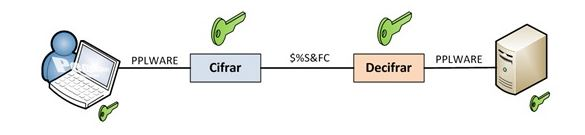
\includegraphics[]{Simetrica.JPG}
	\caption{Funcionamento Criptografia Simétrica}
	\label{cripto1}
\end{figure}

\subsection{Algoritmos de Criptografia Simétrica}
    Os algoritmos  DES , 3DES e AES são alguns dos que utilizam a criptografia simétrica. Podemos analisar outros algoritmos  de  chave  privada  ou  criptografia  simétrica  de  forma  resumida  na Tabela \ref{tab1}:
    
\begin{table}[!h]
\caption{Principais algoritmos de chave privada ou criptografia simétrica}
\label{tab1}
\begin{tabular}{|l|l|l|}
\hline
Algoritmo & Bits                                                     & Descrição                                                                                                                                           \\ \hline
AES       & 128                                                      & \begin{tabular}[c]{@{}l@{}}O Advanced Encryption Standard (AES) é uma cifra de bloco, \\ anunciado pelo National Institute of Standards and Technology (NIST) \\ em  2003,  fruto  de  concurso  para  escolha  de  um  novo algoritmo  \\ de  chave  simétrica  para  proteger  informações  do governo federal, \\ sendo adotado como padrão pelo governo dos Estados  Unidos,  é  \\ um  dos  algoritmos  mais  populares,  desde 2006, usado   para   \\ criptografia   de   chave   simétrica,   sendo considerado como o \\ padrão substituto do DES. O AES tem um tamanho de bloco fixo em \\ 128 bits e uma chave com tamanho de 128, 192 ou 256 bits, ele é \\ rápido tanto em software quanto em hardware, é relativamente fácil \\ de executar e requer pouca memória.\end{tabular}   \\ \hline \end{tabular}  \end{table}

\begin{table}[!h]
\begin{tabular}{|l|l|l|}
\hline 
DES       & 56                                                       & \begin{tabular}[c]{@{}l@{}}O  Data  Encryption  Standard  (DES)  foi  o  algoritmo  simétrico mais  \\ disseminado  no mundo,  até  a  padronização  do  AES.  Foi criado  \\ pela  IBM  em  1977  e,  apesar  de  permitir  cerca  de  72 quadrilhões \\ de combinações, seu tamanho de chave (56 bits) é considerado pequeno, \\ tendo sido quebrado por "força bruta" em 1997 em um desafio lançado na \\ Internet. O NIST que lançou o desafio  mencionado,  recertificou  o  DES  \\ pela  última  vez  em 1993, passando então a recomendar o 3DES.\end{tabular} \\ \hline  
3DES      & \begin{tabular}[c]{@{}l@{}}112 \\ ou \\ 168\end{tabular} & \begin{tabular}[c]{@{}l@{}}O 3DES é uma simples variação do DES, utilizando o em três ciframentos  \\ suscessivos,  podendo  empregar  uma  versão  com duas ou com três \\ chaves diferentes. É seguro, porém muito lento para ser um algoritmo \\ padrão.\end{tabular}                                                                                                                                                                                                                                                                                                                                                                                                                                                                                                                       \\ \hline
IDEA      & 128                                                      & \begin{tabular}[c]{@{}l@{}}O  International Data Encryption Algorithm (IDEA) foi  criado em  1991  \\ por  James  Massey  e  Xuejia  Lai  e  possui  patente  da suíça  ASCOM  \\ Systec.  O  algoritmo  é  estruturado  seguindo  as mesmas linhas  gerais do \\ DES. Mas    na   maioria    dos microprocessadores,  uma   implementação  \\ por   software   do IDEA  é  mais  rápida  do  que  uma  implementação  por  \\ software do  DES.  O  IDEA  é  utilizado  principalmente  no  mercado \\ financeiro  e  no  PGP,  o  programa  para  criptografia  de  e-mail pessoal \\ mais disseminado no mundo.\end{tabular}                                                                                                                                                                \\ \hline
\end{tabular}
\centering Fonte:\cite{STALLINGS:14}
\end{table}




\subsection{Criptografia Assimétrica}

A  criptografia assimétrica,conhecida  por  criptografia de  chaves  públicas, faz p  uso  de  pares  de  chaves  para criptografar ou descriptografar. As duas chaves  são  relacionadas  através  de  um  processo  matemático, usando  funções  unidirecionais para a codificação da informação. A chave pública que, como o nome já diz, qualquer um pode conhecer e ter acesso, é usada para cifrar, enquanto a chave privada, é usada para decifrar. Uma mensagem cifrada com uma chave pública somente poderá ser decifrada com o uso da chave privada com a qual está  relacionada. O método  traz segurança, pois não é necessário compartilhar a chave privada. Em contrapartida, o tempo de processamento de mensagens com criptografia assimétrica é muito maior do que com criptografia simétrica \cite{BURNETT:02}. 
Na FIGURA \ref{cripto2} é demonstrado o processo.

 \begin{figure}[H]
	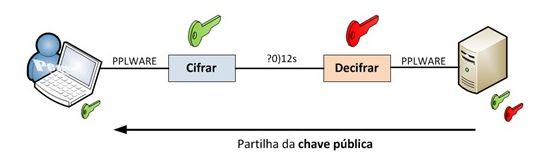
\includegraphics[]{assimetrica.JPG}
	\caption{Funcionamento Criptografia assimétrica}
	\label{cripto2}
\end{figure}

\subsection{Algoritmos de Criptografia Assimétrica}

A grande dificuldade deste sistema é a  complexidade  no  desenvolvimento  dos algoritmos que devem reconhecer a dupla de chaves existentes e relacionar as  mesmas  no  momento  certo,  o  que reverte num  grande  poder  de  processamento computacional para este trabalho \cite{STALLINGS:14}. A  analise  dos  principais  algoritmos  de  chave pública ou criptografia assimétrica de forma resumida na TABELA \ref{tab2}.

\begin{table}[H]
\caption{Principais algoritmos de chaves públicas ou criptografia assimétrica}
\label{tab2}
\begin{tabular}{|l|l|}
\hline
Algoritmo                                                  & Descrição                                                                                                                                                                                                                                                                                                                                                                                                                                                                                                                                                                                                                                                                                                                                                                                                                                                                                                                                                                                                                                                                                                                                                                                                                                                                                                                                                                                                                                                                                                                                                                                                                                                                                                                                                                                                                                                                                                                                                                              \\ \hline
RSA                                                        & \begin{tabular}[c]{@{}l@{}}O RSA  é  um algoritmo  assimétrico  que  possui  este  nome  devido  a  seus \\ inventores:  Ron  Rivest,  Adi Shamir  e  Len  Adleman,  que  o  criaram  em \\ 1977   no   MIT.   Atualmente,   é   o   algoritmo   de   chave   pública   mais \\ amplamente  utilizado,  além  de  ser  uma  das  mais  poderosas  formas  de \\ criptografia  de  chave  pública  conhecidas  até  o  momento.  O  RSA  utiliza \\ números  primos.  A  premissa  por  trás  do  RSA  consiste  na  facilidade  de \\ multiplicar dois números primos para obter um terceiro número, mas muito \\ difícil de recuperar os dois primos a partir daquele terceiro número. Isto é \\ conhecido como fatoração. Por exemplo, os fatores primos de 3.337 são 47 \\ e  71.  Gerar  a  chave  pública  envolve  multiplicar  dois  primos  grandes; \\ qualquer  um  pode  fazer  isto.  Derivar  a  chave  privada  a  partir  da  chave \\ pública  envolve  fatorar  um  grande  número.  Se  o  número  for  grande  o \\ suficiente  e  bem  escolhido,  então  ninguém  pode  fazer  isto  em  uma \\ quantidade  de  tempo  razoável.  Assim,  a  segurança  do  RSA  baseia  se  na \\ dificuldade  de  fatoração  de  números  grandes.  Deste  modo,  a  fatoração \\ representa   um   limite   superior   do   tempo   necessário   para   quebrar   o \\ algoritmo. Uma chave RSA de 512 bits foi quebrada em 1999 pelo Instituto \\ Nacional  de  Pesquisa  da  Holanda,  com  o  apoio  de  cientistas  de  mais  6 \\ países. Levou cerca de 7 meses e foram utilizadas 300 estações de trabalho \\ para a quebra. No Brasil, o RSA é utilizado pela ICP-Brasil, no seu sistema \\ de emissão de certificados digitais, e a partir do dia 1º de janeiro de 2012, \\ as  chaves  utilizadas  pelas  autoridades  certificadoras  do  país,  passam  a \\ serem  emitidas  com  o  comprimento  de  4.096bits,  em  vez  dos  2.048bits \\ atuais.\end{tabular} \\ \hline
ElGamal                                                    & \begin{tabular}[c]{@{}l@{}}O   El Gamal   é   outro   algoritmo   de   chave   pública   utilizado   para \\ gerenciamento de chaves. Sua matemática difere da utilizada no RSA, mas \\ também  é  um  sistema  comutativo.  O  algoritmo  envolve  a  manipulação \\ matemática  de  grandes  quantidades  numéricas.  Sua  segurança  advém  \\ de algo  denominado  problema  do  logaritmo  discreto.  Assim,  o  ElGamal \\ obtém sua segurança da dificuldade de calcular logaritmos discretos em um \\ corpo finito, o que lembra bastante o problema da fatoração.\end{tabular}          \\ \hline                                                                                                                                                                                                                                                                                                  \end{tabular}  \end{table}

\begin{table}[H]
\begin{tabular}{|l|l|l|}
\hline 
\begin{tabular}[c]{@{}l@{}}Diffie -\\ Hellman\end{tabular} & \begin{tabular}[c]{@{}l@{}}Também baseado no problema do logaritmo discreto, e o criptosistema de \\ chave pública mais antigo ainda em uso. O conceito de chave pública, aliás \\ foi  introduzido  pelos  autores  deste  criptosistema em 1976.  Contudo,  ele \\ não permite nem ciframento nem assinatura digital. O sistema foi projetado \\ para permitir a dois indivíduos entrarem em um acordo ao compartilharem \\ um  segredo  tal  como  uma  chave,  muito  embora  eles  somente  troquem \\ mensagens em público.\end{tabular}                                                                                                                                                                                                                                                                                                                                                                                                                                                                                                                                                                                                                                                                                                                                                                                                                                                                                                                                                                                                                                                                                                                                                                                                                                                                                                                                                                                                                                         \\ \hline
\end{tabular}
\centering Fonte: \cite{STALLINGS:14}
\end{table}

\section{Aplicação}
% CRIPTOGRAFIA SIMÉTRICA – utiliza apenas uma chave. Esta chave é utilizada tanto para criptografar quanto para descriptografar a mensagem.
% CRIPTOGRAFIA ASSIMÉTRICA – Utiliza duas chaves. Uma pública e outra privada. A mensagem criptografada por uma chave publica só pode ser descriptografada por uma chave privada correspondente.

Nessa seção será apresentado a utilização da comunicação criptografada para \textbf{\textit{IoT}} em um ambiente usual.


\subsection{Ferramentas De Mercado}

Com os aplicativos sendo parte da rotina dos usuários, visto que o uso é bastante frequente, é mais do que normal que as empresas invistam em segurança. Neste contexto, acaba figurando a criptografia dos apps. Nos dias atuais, o mecanismo foi empregado de modo a proteger os dados dos usuários, sobretudo de invasores. O sistema Android, por exemplo, já oferece essa tecnologia em sua linguagem de programação, e aplicativos como o WhatsApp, Telegram, e \textit{\textbf{Followzup }}por exemplo, são  alguns dos que usam a criptografia em sua comunicação.

No geral, o sistema do aplicativo codifica informações do próprio aparelho, de modo a impedir que hackers invadam os dados e as usem de modo indevido. Resumindo, há uma espécie de chave colocada pelo próprio usuário que impede o uso desses dados. Essa proteção vai muito além das senhas de desbloqueio do aparelho, já que são mantidas por aplicativos.


\subsection{Followzup}

O \textit{\textbf{Followzup }}é um serviço gratuito para envio de mensagens de texto criptografadas para celulares e outros dispositivos móveis. As mensagens são enviadas em background, a partir de sistemas e websites com o auxílio de APIs, disponíveis em PHP, Java, Ruby, Perl, Python,  C\# e .NET. As APIs são simples de usar, e com apenas 1 linha de comando a aplicação pode enviar uma mensagem para o celular de um ou mais usuários \cite{followzup}.


Além de enviar, os websites Internet também podem receber mensagens dos usuários, originadas a partir de seus dispositivos móveis. A comunicação entre sistemas e dispositivos móveis por meio do \textit{\textbf{Followzup }}é criptografada com os padrões AES e RSA, e o protocolo aberto do serviço permite o desenvolvimento de APIs para outras linguagens, assim como o desenvolvimento de APPs para diferentes modelos de dispositivos móveis \cite{followzup}.

Exemplos de uso:
\begin{itemize}
    \item Monitorar a atividade de usuários em sistemas e websites;
    \item Monitorar e enviar alertas sobre ocorrências em sistemas e equipamentos;
    \item Enviar notícias, dicas, avisos e mensagens publicitárias;
    \item Receber mensagens de solicitações dos usuários;
    \item Solicitar respostas de confirmação dos usuários;
    \item Enviar mensagens associadas a “links” externos;
    \item Informar e confirmar agendamento de compromissos;
    \item Informar a realização transações comerciais e financeiras;
    
\end{itemize}

As mensagens enviadas por meio do \textit{\textbf{Followzup }}são criptografadas com os protocolos AES e RSA, garantindo confidencialidade em todo o trajeto percorrido pela informação. Cada aplicação e cada dispositivo móvel possui seu próprio par de chaves assimétricas RSA, e apenas o webservice \textit{\textbf{Followzup }}pode decriptografar e ter acesso ao conteúdo das requisições. A figura \ref{parDeCha} representa o modelo de criptografia utilizado pelo Followzup.

 \begin{figure}[H]
 \centering
	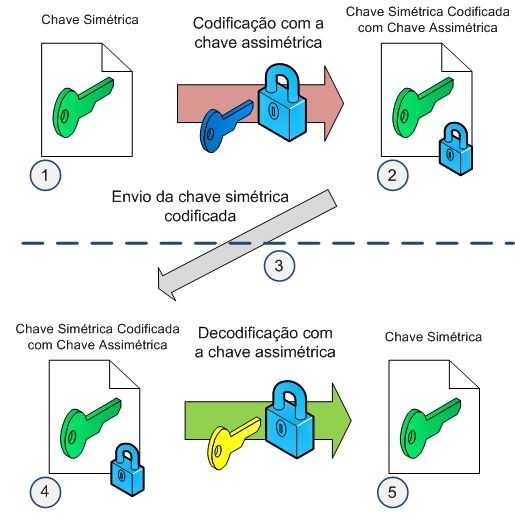
\includegraphics[scale=0.9]{jogoDeChaves.JPG}
	\caption{Modelo de Criptografia RSA e AES}
	\label{parDeCha}
\end{figure}


Cada solicitação encaminhada ao serviço \textit{\textbf{Followzup }}possui seu próprio número de sequência, garantindo maior segurança na comunicação entre sistemas e dispositivos. Com esse nível adicional de segurança, as requisições eventualmente interceptadas e reenviadas pela rede de acesso, são automaticamente consideradas inválidas pelo serviço \cite{followzup}. O modelo de XML da figura \ref{xml} apresenta uma solicitação encaminhada ao Followzup.

 \begin{figure}[H]
 \centering
	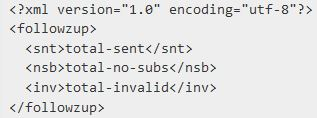
\includegraphics[scale=1]{xml}
	\caption{Resposta de Solicitação FollowZup}
	\label{xml}
\end{figure}

A figura \ref{xml} é um modelo de resposta a uma solicitação \textit{\textbf{Followzup }}onde cada \textbf{TAG} tem aseguinte função:

\begin{itemize}
   
\item \textbf{Total-sent:} Total de mensagens enviadas.
\item \textbf{Total-no-subs:} Total de destinatários informados na solicitação que não são assinantes do canal.
 \item \textbf{Total-invalid:} Total de destinatários informados na solicitação que foram considerados inválidos. 
\end{itemize}

\section{Implementação \textit{\textbf{Followzup }}}

Para que aplicações, websites ou dispositivos possam enviar e receber mensagens eles precisam estar associados a um canal de comunicação. A criação do canal de comunicação deve ser realizada no site do \textit{\textbf{Followzup }}por um usuário previamente cadastrado, tal canal pertencera ao usuário que o criou. Um canal não pode ser compartilhado por dois usuários pois implicaria em falha de segurança.
Após criar o canal será fornecido o par de chaves RSA para uso exclusivo do canal, usadas para transmissão de dados criptografados pelo canal, cabe ao desenvolvedor realizar o download da api com o par de chaves RSA e aplica-las ao produto.



No \textit{\textbf{Followzup }}existe três maneiras de transmitir uma mensagem, elas podem ser enviadas em  broadcast, quando uma mesma mensagem e enviada a todos os usuários de um canal de comunicação. A segunda forma é o unicast, utilizada Para transmitir a mensagem para somente um usuário. A terceira forma é a que multicast, onde uma mensagem é transmitida a um determinado grupo de assinantes de um canal de comunicação.



A identificação do usuário pode ser realizada pelo e-mail ou pelo user-ID. Um outro parâmetro fornecido é o tempo de vida da mensagem de uma mensagem, em situações que o aparelho ou aplicação fiquem fora de serviço a aplicação emissora da mensagem pode delimitar um tempo de vida em horas para uma mensagem ser entregue.


Para enviar as mensagens as aplicações devem chamar o método submit contida na API. A figura \ref{java1} abaixo implementa o envio de uma mensagem utilizando o método submit da api do followzap na tecnologia Java.


 \begin{figure}[H]
 \centering
	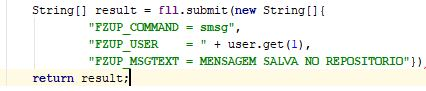
\includegraphics[scale=1]{javacode.JPG}
	\caption{Enviando Mensagem Followzap}
	\label{java1}
\end{figure}

A tabela \ref{comands} apresenta os comandos que podem ser utilizados no envio de uma mensagem.
\begin{table}[H]
\centering
\caption{Parametros de Envio de Mensagens}
\label{comands}
\begin{tabular}{|l|l|l|}
\hline
ZUP\_COMMAND                 & Obrigatório                  & \begin{tabular}[c]{@{}l@{}}Deve conter a literal smsg \\ (send message).\end{tabular}                                                                                                                           \\ \hline
FZUP\_LASTSEQ                & Opcional                     & \begin{tabular}[c]{@{}l@{}}Contém o número de sequência \\ da última solicitação.\end{tabular}                                                                                                                  \\ \hline
\multirow{7}{*}{FZUP\_USER}  & \multirow{7}{*}{Obrigatório} & Contém o destinatário da mensagem:                                                                                                                                                                              \\ \cline{3-3} 
                             &                              & \begin{tabular}[c]{@{}l@{}}Literal “all”, para enviar mensagem \\ a todos os assinantes (broadcast).\end{tabular}                                                                                               \\ \cline{3-3} 
                             &                              & \begin{tabular}[c]{@{}l@{}}E-mail ou User-ID do assinante, para \\ enviar mensagem a um único \\ destinatário (unicast).\end{tabular}                                                                           \\ \cline{3-3} 
                             &                              & \begin{tabular}[c]{@{}l@{}}Ex: e-mail: “user.mail@anymail.com”, \\ User-ID: “z12h49d934jw”.\end{tabular}                                                                                                        \\ \cline{3-3} 
                             &                              & \multirow{2}{*}{\begin{tabular}[c]{@{}l@{}}Lista com até 200 e-mails ou User-IDs \\ separados por vírgulas, para \\ grupos de assinantes (multicast).\end{tabular}}                                             \\ 
                             &                              &                                                                                                                                                                                                               \\&  & \\ \hline 
\multirow{2}{*}{FZUP\_HOURS} & \multirow{2}{*}{Opcional}    & \begin{tabular}[c]{@{}l@{}}Deve conter um valor numérico entre \\ 1 e 960, representando o \\ tempo de vida da mensagem em horas.\end{tabular}                                                                  \\ \cline{3-3} 
                             &                              & \begin{tabular}[c]{@{}l@{}}Para os valores inválidos ou não \\ informados, o tempo de \\ vida será definido em 24 horas.\end{tabular}                                                                           \\ \hline
FZUP\_MSGTEXT                & Obrigatório                  & \begin{tabular}[c]{@{}l@{}}Deve conter a mensagem a ser \\ enviada, com até 200 caracteres.\end{tabular}                                                                                                        \\ \hline
FZUP\_MSGURL                 & Opcional                     & \begin{tabular}[c]{@{}l@{}}Contém o endereço HTTP que será \\ utilizado como “link” associado à mensagem, \\ permitindo que o destinatário abra a URL \\ informada ao clicar no texto da mensagem.\end{tabular} \\ \hline
\end{tabular}
FONTE: \cite{followzup}
\end{table}
As mensagens enviadas por usuários de aplicações chegam por meio de um post em suas respectivas URL de destino contendo duas variáveis: 
\begin{itemize}
    \item \textbf{fzupidchannel:}  	Identificação do canal que está recebendo a mensagem (não criptografado).
    \item \textbf{fzupresponse:}  	String contendo a data/hora, User-ID e mensagem do usuário (criptografado). 
\end{itemize}

A figura \ref{java2} apresenta o recebimento de uma mensagem \textit{\textbf{Followzup }}em um servidor, extraindo a string criptografada de um cabeçalho HTTP, logo em seguida e feita a de criptografia utilizando o método \textbf{decrypt} da api:

 \begin{figure}[H]
 \centering
	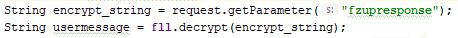
\includegraphics[scale=1]{javacode2.JPG}
	\caption{Recebendo Mensagem Followzap}
	\label{java2}
\end{figure}


Conteúdo da string:
\begin{itemize}
\item YYYY-MM-DD HH:MM:SS;User-ID;Text-message
\end{itemize}


Onde:
\begin{itemize}
\item YYYY-MM-DD HH:MM:SS = Data e hora de envio da mensagem
\item User-ID = Identificação do usuário
\item Text-message = Texto da mensagem
\end{itemize}


\subsection{Api Rest Followzap}

Utilizando os conhecimentos adquiridos durante a elaboração deste trabalho foi implementado uma solução de comunicação criptografada utilizando o canal de comunicação Followzup e a aplicação mobile Followzup. 

O resultado foi uma API REST implementada em Java utilizando o Framework Spring-Boot. A aplicação tem como funcionalidade:
\begin{itemize}
 
\item  Armazenar mensagens enviadas por um usuário assinante do canal.
\item  Listar as mensagens salvas quando o usuário solicitar.
   
\end{itemize}{}
As mensagens devem ser enviadas pelo aplicativo do Followzup, encontrado nas lojas de aplicações mobile. O servidor está armazenado em uma aplicação Heroku que fornece um ambiente de trabalho idêntico ao real quando se trabalha com comunicação pela internet. 


O pacote de códigos fonte podem ser baixados no link: \textit{\textbf{https://github.com/ErikZA/appRestComunicacaoCriptografada}}.


\section{Conclusão}

Com a evolução da tecnologia e cada vez mais dispositivos conectados a internet a utilização de modelos de segurança para proteção dos dados é essencial. Tem-se como exemplo todas as metodologias e técnicas de criptografia que foram mostradas ao longo do item 2 para a proteção dos dados que trafegam pela internet. 

Cedo ou tarde todas as chaves de criptografia foram quebradas, ou seja, utilizar da criptografia não garante totalmente a segurança dos dados, porém nenhuma outra técnica de segurança da informação é tão eficaz quanto a criptografia. Por isso, pode-se afirmar a criptografia é a melhor forma de proteção contra o vazamento de dados.


Aplicações proposta por este trabalho, aumenta substancialmente a segurança de sistemas e usuários garantindo a  ocultação dos dados de comunicação entre sistemas através de chaves criptográficas e canais de comunicação encriptografados. Desta forma torna-se o trabalho de invadir estes sistemas mais custos do que as informações que serão obtidas ao tentar invadi-lo. 

A adoção de modelos como estes por empresas, usuários e acadêmicos fara da \textit{\textbf{IoT}} uma tecnologia mais segura e mais rentável pois cada vez mais pessoas e instituições buscarão os benefícios da comunicação segura pela \textit{\textbf{IoT}}.






\bibliographystyle{sbc}
\bibliography{sbc-template}

\end{document}
